\documentclass{beamer}
\usepackage{beamerthemeshadow}
\usepackage{beamercolorthemedolphin}
\usepackage{lastpage}

\usepackage{xcolor}
\usepackage{pgf}

\newcommand{\bi}{\begin{itemize}}
\newcommand{\ei}{\end{itemize}}
\newcommand{\be}{\begin{enumerate}}
\newcommand{\ee}{\end{enumerate}}
\newcommand{\bd}{\begin{description}}
\newcommand{\ed}{\end{description}}
\newcommand{\prbf}[1]{\textbf{#1}}
\newcommand{\prit}[1]{\textit{#1}}
\newcommand{\beq}{\begin{equation}}
\newcommand{\eeq}{\end{equation}}
\newcommand{\bdm}{\begin{displaymath}}
\newcommand{\edm}{\end{displaymath}}

\newcommand{\ft}[1]{
  \frametitle{\begin{tabular}{p{4in}r} #1 & \small{\textcolor{white}{\thepage$~$ / \pageref{LastPage}}}\end{tabular}}
  \setbeamercovered{transparent=18}
}

\newcommand{\stepinv}{\setbeamercovered{invisible}}
\newcommand{\stopinv}{\setbeamercovered{transparent=18}}
\newcommand{\uncoverinv}[1]
{
  \setbeamercovered{invisible}
  \uncover<+->{#1}
  \setbeamercovered{transparent=18}
}
\newcommand{\ans}[1]{\textcolor{blue}{#1}}
\newcommand{\ansinv}[1]
{
  \setbeamercovered{invisible}
  \uncover<+->{\textcolor{blue}{#1}}
  \setbeamercovered{transparent=18}
}
\newcommand{\setinv}{\setbeamercovered{invisible}}
\newcommand{\setvis}{\setbeamercovered{transparent=18}}
\newcommand{\centerpic}[2]
{
  \begin{center}
  \includegraphics[#1]{#2}
  \end{center}
}
\newcommand{\h}[1]{\hat{#1}}
\newcommand{\ds}{\displaystyle}

\definecolor{mycolor}{rgb}{0.125,0.5,0.05}
\definecolor{newcolor}{rgb}{0.75,0.40,0.0}
\usecolortheme[named=mycolor]{structure}

\title[Empirical Significance of Learning with Firm-Specific Capital]{Empirical Significance of Learning in a New Keynesian Model with Firm-Specific Capital}
\author[Macro Group Workshop.  Indiana University.  February 2007.]{James Murray}
\date{February 2, 2007}

\begin{document}

\frame{\titlepage}
\setcounter{page}{1}

\frame{
  \ft{Motivation for Learning}
  \bi
  \item Least squares learning: no rational expectations, instead agents form all expectations using least squares estimates.
  \item Orphanides and Williams (2005): inflation scares.
  \item Primiceri (2005): High inflation (1970s) followed by dis-inflation (1980s).
  \item Milani (2005): Learning, not habit formation or inflation indexation, explains persistence.
  \item Mark (2005): Dollar / DM real exchange rate depreciation (1970s), appreciation (early 1980s), depreciation (late 1980s).
  \ei
}

\frame
{
  \ft{Motivation for Estimation}
  \bi
  \item All these results depend on the size of the learning gain.
  \item Milani (2005) finds a statistically significant learning gain with a 3 equation NKPC model.
  \item Learning provides a better fit to the data:
    \bi
    \item Allows for greater persistence.
    \item Allows for time varying volatility.
    \ei
  \item Is learning significant because the model is too simple?
  \item Contribution: estimate with endogenous firm-specific capital (Woodford, 2005).
  \ei
}

\frame
{
  \ft{Motivation for Endogenous Capital}
  \bi
  \item Introduces an additional source of persistence.
  \item Affects how agents make expectations.
  \item Evolution of output and inflation depend on investment decisions.
  \item Additional data for estimation: investment.
  \ei
}

\frame
{
  \ft{Overview}
  \bi
  \item Goals:
    \bi
    \item Find out whether adding capital is important.
    \item Find out if learning is statistically significant with more general model.
    \item Find out what dynamics of U.S. data learning helps explain.
    \ei
  \item Method:
    \bi
    \item Examine impulse response functions with/without capital.
    \item Estimate NK model with capital and learning by MLE.
    \item Examine the forecast errors.
    \ei
  \item Findings:
    \bi
    \item Capital makes a difference.
    \item Learning remains statistically significant.
    \item Learning helps explain volatility.
    \item Learning + capital best able to explain U.S. experience.
    \ei
  \ei
}

\frame
{
  \ft{Outline}
  \be
  \item Overview Woodford (2005) model.
  \item Overview of learning in DSGE model.
  \item Present impulse responses.
  \item Present estimation results.
  \item Conclude.
  \ee
}

\frame
{
  \ft{Model}
  \bi
  \item Continuum of consumer types, each type supplies a unique type of labor.
  \item Consumers exhibit habit formation.
  \item One final good produced in a perfectly competitive market.
  \item Final good produced with a continuum of intermediate goods.
  \item Intermediate goods each hire specific labor, require a firm-specific capital good.
  \item Intermediate goods firms are monopolistically competitive.
  \item Calvo (1983) pricing for intermediate goods.
  \ei
}

\frame
{
  \ft{Consumers}
  \textbf{Utility function:}
  \bdm U_0 = E_0 \sum_{t=0}^{\infty} \beta^t \left[ \frac{1}{1-\sigma} \xi_t \left(c_t - \eta c_{t-1}\right)^{1-\sigma} - \frac{1}{1+\mu} n_t(i)^{1+\mu} \right] \edm
  \bi
  \item $c_t$: consumption at time $t$. 
  \item $n_t(i)$: labor supply at time $t$.
  \item $\xi_t$: common preference shock.
  \item $\beta$: discount factor.
  \item $\sigma \in (0,\infty)$: related to the intertemporal elasticity of substitution.
  \item $\eta \in [0,1)$: degree of habit formation.
  \ei
}

\frame
{
  \ft{Demand side of model}
  Utility maximization + log-linearization:
  \bdm \h{\lambda}_{t} = E_t \h{\lambda}_{t+1} + \h{r}_t - E_t \pi_{t+1} \edm
  \bdm \h{\lambda}_t = \frac{1}{ (1-\beta \eta)(1-\eta)}\left[ \beta \eta \sigma E_t \h{c}_{t+1} - \sigma(1+\beta \eta^2) \h{c}_t + \sigma \eta \h{c}_{t-1} \right] + \h{\xi}_t \edm
  \bi
  \item Hats denote percentage deviations from steady state.
  \item $\lambda_t$ is Lagrange multiplier = marginal utility of income.
  \item Note: habit formation adds a ``mechanical'' source of persistence.
  \ei
}

\frame
{
  \ft{Production}
  \textbf{Final good production:}
  \bdm y_t = \left[ \int_0^1 y_t(i)^{\frac{\theta-1}{\theta}} di \right]^{\frac{\theta}{\theta-1}} \edm
  \bi
  \item $y_t$ output of final good, $y_t(i)$ output of intermediate good $i$.
  \item $\theta \in (1,\infty)$: elasticity of substitution in production.
  \ei
  \textbf{Intermediate goods production:}
  \bdm y_t(i) = z_t k_t(i)^{\alpha} n_t(i)^{1-\alpha} \edm
  \bi
  \item $z_t$: common technology shock.
  \item $k_t(i)$: firm-specific capital good.
  \ei
}

\frame
{
  \ft{Sticky prices}
  \bi
  \item Follow Calvo (1983) pricing.
  \item Even with endogenous capital (Woodford, 2005), leads to standard looking Phillips curve:
  \bdm \pi_t = \beta E_t \pi_{t+1} + \kappa \h{s}_t \edm
  \item $s_t$: average marginal cost in the economy.
  \item $\kappa$: function of many parameters.
    \bi 
    \item No closed form expression when there is endogenous capital.
    \item Increasing with degree of price flexibility.
    \ei
  \ei
}

\frame
{
  \ft{Firm-Specific Investment}
  \bi
  \item Final good is converted to a firm-specific capital good.
  \item Investment of $I_t(i)$ leads to capital stock next period:
  \ei
  \bdm k_{t+1}(i) = (1-\delta) k_t(i) + \mu_t I_t(i) - \frac{\phi}{2} \left[\frac{k_{t+1}(i)}{k_t(i)} - 1 \right]^2 k_t(i) \edm
  \bi
  \item $\mu_t$: common investment technology shock.
  \item $\delta$: depreciation rate.
  \item $\phi$: capital adjustment cost parameter.
  \ei
}

\frame
{
  \ft{Log-linear supply relationships}
  \bi
  \item Optimal demand for labor and capital:
  \bdm \h{s}_t = \frac{\mu+\alpha}{1-\alpha} \h{y}_t - \frac{\alpha(\mu+1)}{1-\alpha} \h{k}_t - \h{\lambda}_t - \frac{\mu+1}{1-\alpha} \h{z}_t \edm
  \item Optimal investment:
  \bdm \label{eq:lneqk} \begin{array}{l}
\ds \h{\lambda}_t + \phi \left(\h{k}_{t+1} - \h{k}_t\right) = \ds \beta (1-\delta) E_t \h{\lambda}_{t+1} \\ \\
\ds + \left(\frac{1-\beta \left(1-\delta \right)}{1-\alpha} \right) \left[ (\mu+1) E_t \h{y}_{t+1} - (1+\alpha \mu) \h{k}_{t+1}\right] \\ \\ 
\ds + \beta \phi \left(E_t\h{k}_{t+2} - \h{k}_{t+1}\right) + \h{\mu}_t 
  \end{array} \edm
  \ei
}

\frame
{
  \ft{Market clearing / Monetary Policy}
  \textbf{Log-linear market clearing condition:}
  \bdm \h{y}_t = c_y \h{c}_t + \delta k_y \h{I}_t \edm
  \bi
  \item $c_y$: steady state consumption / output ratio.
  \item $k_y$: steady state capital / output ratio.
  \ei
  \textbf{Monetary policy}:
  \bdm \h{r}_t = \rho_r \h{r}_{t-1} + (1-\rho_r) \left(\psi_{\pi} \pi_t + \psi_y \h{y}_t \right) + \epsilon_{r,t} \edm
  \bi
  \item $\psi_{\pi} \in (0,\infty)$: feedback on inflation.
  \item $\psi_{y} \in (0,\infty)$: feedback on output.
  \item $\rho_r \in (0,1)$: smoothing parameter.
  \ei
}

\frame
{
  \ft{Structural shocks}
  \bi
  \item There are four structural shocks in the model:
    \bi
    \item $\h{\xi}_t$: preference shock
    \item $\h{z}_t$: technology shock
    \item $\h{\mu}_t$: investment shock
    \item $\h{\epsilon}_{r,t}$: monetary policy shock
    \ei
  \item Assume shocks are all iid normally distributed with no serial correlation.
    \bi
    \item Serial correlation would definitely fit data better.
    \item Purpose: explain which \textit{economic explanations} explain U.S. data.
    \item Look at forecast errors.
    \ei
  \ei
}

\frame
{
  \ft{Learning in DSGEs}
  \bi
  \item Agents do not know any parameters of the model.
  \item Expectations are all replaced by least squares forecasts.
  \item Timing:
    \be
    \item Beginning of period $t$: data is collected through period $t+1$.
    \item Agents compute least squares forecasts.
    \item Based on expectations, make consumption, production, investment, pricing decisions.
    \item End of time $t$: time $t$ observations are realized.
    \ee
  \item Timing is both realistic, incredibly convenient.
  \ei
}

\frame
{
  \ft{A General Model}
  Suppose a DSGE model of the form:
  \bdm \Omega_{0} x_t = \Omega_{1} x_{t-1} + \Omega_{2} E_t^* x_{t+1} + \Psi \epsilon_t \edm
  \bi
  \item $x_t$ vector of time $t$ variables, all observable to agents.
  \item $E_t^*$: possibly non-rational expectations operator.
  \ei
  \vspace{1pc}
  Rational expectations solution implies:
  \bdm E_t x_{t+1} = G x_t \edm
  \bi
  \item Agents know the form of this solution, but estimate elements of $G$ by least squares.
  \item Use as explanatory variables past observations of $x_t^k$.
  \item $x_t^k$ includes all variables in $x_t$ where the associated column in $G$ is non-zero.
  \ei
}
  
\frame
{
  \ft{Ordinary Least Squares}
  \bi 
  \item Let $G_t^k$ denote non-zero columns of $G$.
  \item Ordinary least squares estimate for $G^k$ at time $t$:
    \bdm \left(\hat{G}_t^k\right)' = \left( \frac{1}{t-1} \sum_{\tau=1}^{t-1} x_{\tau-1}^k {x_{\tau-1}^{k}}' \right)^{-1} \left( \frac{1}{t-1} \sum_{\tau=1}^{t-1} x_{\tau-1}^k x_{\tau}' \right) \edm
  \item Least squares forecast:
  \bdm E_t^* x_{t+1} = \h{G}_t E_t^* x_t = \h{G}_t^2 x_{t-1} \edm
  \item Evolution of $\h{G}_t$ in recursive form:
    \bdm \hat{G}_t^k = \hat{G}_{t-1}^k + g (x_{t-1} - \hat{G}_{t-1} x_{t-2}) {x_{t-2}^k}' R_t^{-1} ,\edm
    \bdm \label{eq:lnX} R_t = R_{t-1} + g (x_{t-2}^k {x_{t-2}^k}' - R_{t-1}) \edm
  \item where $g=1/(t-1)$ is the learning gain.
  \ei
}

\frame
{
  \ft{Constant Gain Learning}
  \bi
  \item Ordinary least squares $\rightarrow$ learning dynamics disappear as $t$ grows.
  \item Constant gain: assumes $g$ is constant.
  \item With a constant gain, learning dynamics persist in the long run.
  \item Dynamics of expectations depend on the size of the constant learning gain.
  \item Appropriate initial condition + $(g=0)$ $\rightarrow$ RE.
  \item Standard statistical test for $g=0$ can conclude a rejection failure to RE.
  \ei
}

\frame
{
  \ft{Learning Dynamics}
  \bi
  \item Substitution of the forecast $E_t^* x_{t+1}$ into the structural form:
  \bdm x_t = \Omega_0^{-1} \left(\Omega_{1} + \Omega_{2} \h{G}_t^2 \right) x_{t-1}  + \Omega_0^{-1} \Psi \epsilon_t \edm
  \item This solution is used to generate IRFs, estimate model by MLE.
  \item The impact of $x_{t-1}$ on $x_t$ is time varying.
  \item Depends on expectations, and therefore past data.
  \item Therefore, learning delivers persistence, time varying volatility.
  \ei
}

\frame
{
  \ft{Impulse responses}
  \bi
  \item Technology shock ($z_t$) and a preference shock ($\xi_t$).
  \item Look at case with fixed capital and endogenous capital.
  \item Look at $g=0.05$, and $g=0$.
  \item Response will depend on initial condition for $\h{G}_t$.
  \item Simulate 1000 IRFs with different initial conditions, report quartiles.
  \ei
}

\frame
{
\begin{table}[ht]
\caption{Parameter values used for Impulse Response Functions}\label{tb:calparms}
\begin{small}
\begin{center}
\begin{tabular}{|l|c|c|} \hline
Description & Parameter & Value \\ \hline
Discount rate & $\beta$ & 0.99 \\ 
Learning gain & $g$ & 0.05 \\
Habit formation & $\eta$ & 0.8 \\
Depreciation rate & $\delta$ & 0.025 \\
Inverse elasticity sub. & $\sigma$ & 2 \\ 
Inverse elasticity labor supply & $\mu$ & 1 \\ 
Cost of adjusting capital & $\phi$ & 0.1 \\ 
Elasticity sub. in production & $\theta$ & 4 \\ 
Price flexibility & $\kappa$ & 0.1 \\ 
MP interest rate smoothing & $\rho_r$ & 0.1 \\ 
MP feedback on output & $\psi_y$ & 0.5 \\ 
MP feedback on inflation & $\psi_{\pi}$ & 1.5 \\ 
Std. dev. technology shock & $\sigma_z$ & 0.02 \\ 
Std. dev. investment shock & $\sigma_{\mu}$ & 0.02 \\ 
Std. dev. preference shock & $\sigma_{\xi}$ & 0.02 \\ 
Std. dev. interest rate shock & $\sigma_{r}$ & 0.02 \\ \hline 
\end{tabular}
\end{center}
\end{small}
\end{table}
}

\frame
{
\begin{figure}[ht]
\caption{Technology shock IRF (fixed capital stock)}
\begin{center}
\begin{tabular}{cc}
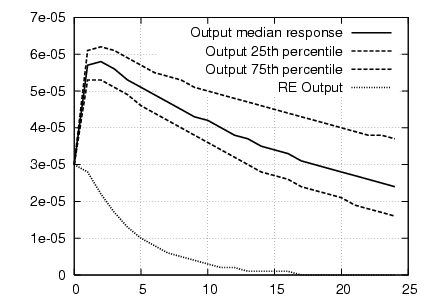
\includegraphics[scale=0.3]{plots/outputirf_znok.png} &
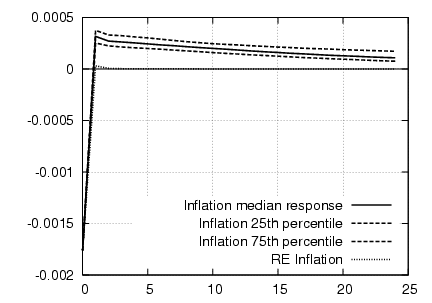
\includegraphics[scale=0.3]{plots/inflationirf_znok.png} \\
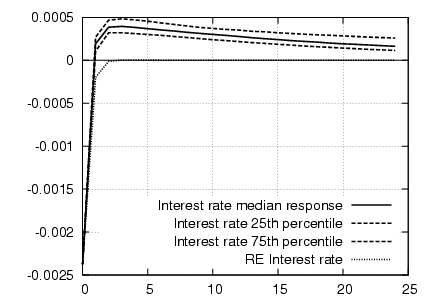
\includegraphics[scale=0.3]{plots/interestirf_znok.png} \\
\end{tabular}
\end{center}
\end{figure}
}

\frame
{
  \ft{Technology shock IRF (fixed capital)}
  \bi
  \item Habit formation causes some persistence.
  \item Increased expectations of future consumption.
  \item Causes an increase in demand for current consumption.
    \bi
    \item Causes prolonged increases in output.
    \item Increase in demand (caused by expectations) causes an \textit{increase} in prices.
    \ei
  \item Expectations take time to return to normal.
  \ei
}

\frame
{
\begin{figure}[ht]
\caption{Technology shock IRF (endogenous capital stock)}
\begin{center}
\begin{tabular}{cc}
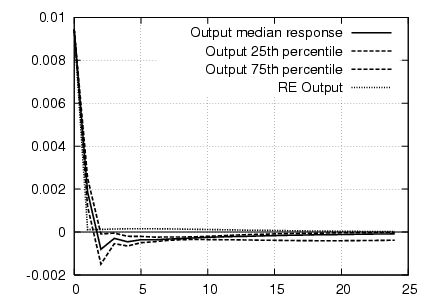
\includegraphics[scale=0.3]{plots/outputirf_z.png} &
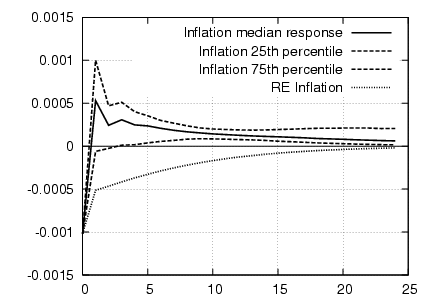
\includegraphics[scale=0.3]{plots/inflationirf_z.png} \\
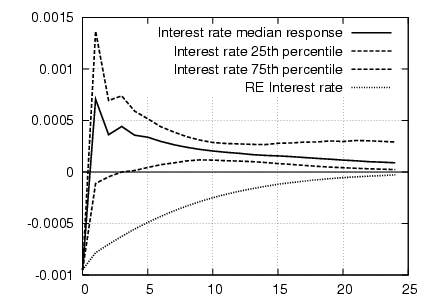
\includegraphics[scale=0.3]{plots/interestirf_z.png} &
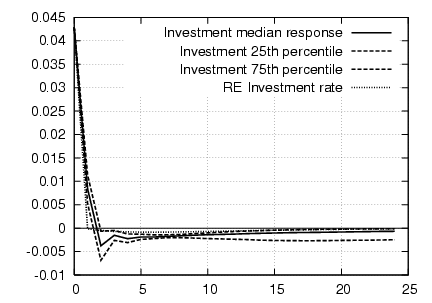
\includegraphics[scale=0.3]{plots/investmentirf_z.png} \\
\end{tabular}
\end{center}
\end{figure}
}

\frame
{
  \ft{Technology shock IRF (endogenous capital stock)}
  \bi
  \item Output response completely different.
  \item Demand side expectations are same.
  \item Supply side expectations: producers expect higher productivity in the future.
  \item Firms increase investment in period of shock AND period following the shock.
  \item Over-investment decreases marginal product of capital, expectations reverse.
  \item Period 3 onward: expectations decrease supply and increase demand.
    \bi
    \item Investment decreases.
    \item Small changes in output.
    \item Prolonged inflation.
    \ei
  \ei
}

\frame
{
\begin{figure}[ht]
\caption{Preference shock IRF (fixed capital stock)}
\begin{center}
\begin{tabular}{cc}
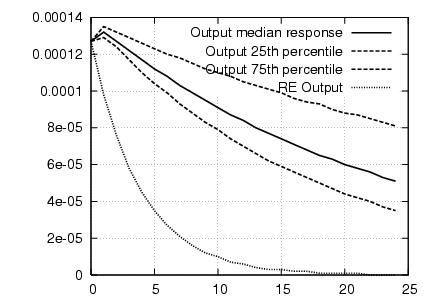
\includegraphics[scale=0.3]{plots/outputirf_xinok.png} &
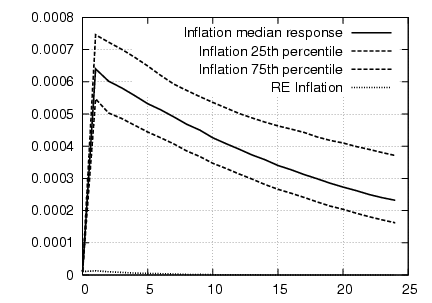
\includegraphics[scale=0.3]{plots/inflationirf_xinok.png} \\
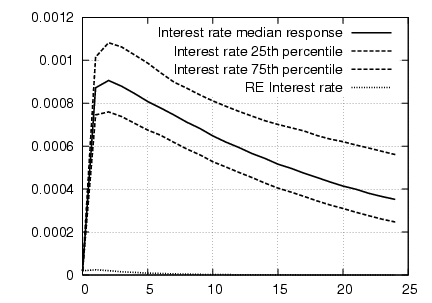
\includegraphics[scale=0.3]{plots/interestirf_xinok.png} \\
\end{tabular}
\end{center}
\end{figure}
}

\frame
{
  \ft{Preference shock IRF (fixed capital)}
  \bi
  \item Habit formation causes some persistence.
  \item Increased expectations of future consumption.
  \item Causes an increase in demand for current consumption.
    \bi
    \item Causes prolonged increases in output.
    \item Increase in demand causes further \textit{increase} in prices.
    \ei
  \item Expectations take time to return to normal.
  \ei
}

\frame
{
\begin{figure}[ht]
\caption{Preference shock IRF (endogenous capital stock)}
\begin{center}
\begin{tabular}{cc}
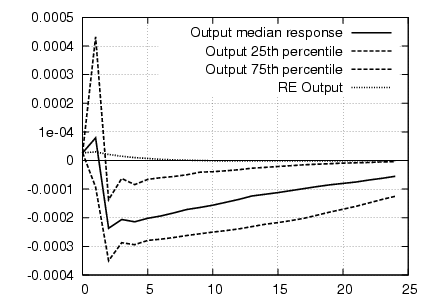
\includegraphics[scale=0.3]{plots/outputirf_xi.png} &
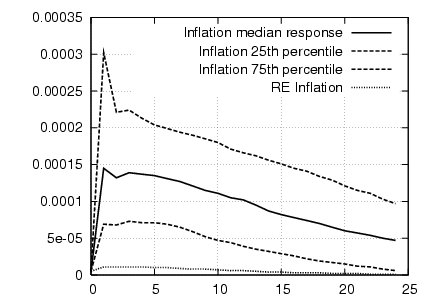
\includegraphics[scale=0.3]{plots/inflationirf_xi.png} \\
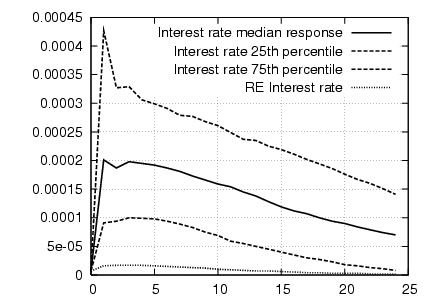
\includegraphics[scale=0.3]{plots/interestirf_xi.png} &
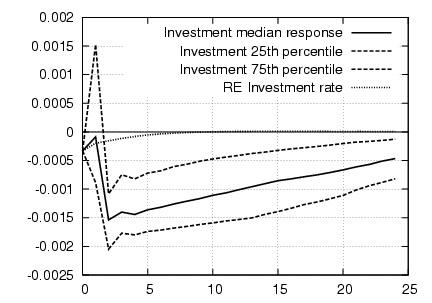
\includegraphics[scale=0.3]{plots/investmentirf_xi.png} \\
\end{tabular}
\end{center}
\end{figure}
}

\frame
{
  \ft{Preference shock IRF (endogenous capital stock)}
  \bi
  \item Output response completely different.
  \item Demand side expectations are same.
  \item Supply side expectations: producers expect higher demand in the future.
  \item Firms over-invest.
  \item Investment decreases.
  \item Small changes in output.
  \item Prolonged inflation.
  \ei
}

\frame
{
  \ft{Estimation: Data}
  Data: quarterly U.S. data from 1957:Q1 through 2005:Q4.
  \bi
  \item Growth rate of real GDP (de-meaned).
  \item Growth rate of real gross private domestic investment (de-meaned).
  \item Annualized inflation rate of CPI.
  \item Annualized federal funds rate.
  \ei
}

\frame
{
  \ft{Estimation Procedure}
  Estimate by MLE using Kalman filter (Hamilton, 1994).
  \bi
  \item State equation: 
  \bdm x_t = \Omega_0^{-1} \left(\Omega_{1} + \Omega_{2} \h{G}_t^2 \right) x_{t-1}  + \Omega_0^{-1} \Psi \epsilon_t \edm
  \item Observation equations:
    \bdm \begin{array}{c} 
      \ds GDP_t^g = 100\left(\h{y}_t - \h{y}_{t-1}\right) \\
      \ds I_t^g = 100\left(\h{I}_t - \h{I}_{t-1}\right) \\
      \ds INF_t^{CPI} = \pi^{*} + 400\pi_t \\
      \ds FF_t = r^{*} + 400\h{r}_t
    \end{array}
    \edm
  \item $\pi^*$: steady state inflation. NK model assumes is zero.
  \item $r^*$: steady state nominal interest rate.
  \ei
}

\frame
{
  \ft{Parameters}
  \bi
  \item Fix $\beta=0.99$, $\delta=0.025$, $\alpha=0.33$.
  \item Maximize likelihood with respect to:
  \bdm \Theta_{1} = [g~\eta~\sigma~\mu~\phi~\theta~\kappa~\rho_r~\psi_y~\psi_{\pi} ~\pi^{*} ~\sigma_z ~\sigma_{\mu} ~\sigma_{\xi} ~\sigma_{r}]' \edm
  \item When estimating the model without capital, $\mu$, $\phi$, $\theta$, and $\sigma_{\mu}$, become unidentifiable.
  \bdm \Theta_{2} = [g~\eta~\sigma~\kappa~\rho_r~\psi_y~\psi_{\pi} ~\pi^{*} ~\sigma_z ~\sigma_{\xi} ~\sigma_{r}]' \edm
  \item Estimate four cases:
    \be
    \item Fixed capital + learning.
    \item Fixed capital + $(g=0)$.
    \item Endogenous capital + learning.
    \item Endogenous capital + $(g=0)$.
    \ee
  \ei
}

\frame
{
\begin{table}[ht]
\caption{MLE Results with Learning and Fixed Capital}
\begin{small}
\begin{center}
\begin{tabular}{|l|c|c|c|c|} \hline
Parameter &  & Estimate & Std. dev. & P-value. \\ \hline
Learning gain & $g$ & 0.008503 & 0.004215 & 0.021818 \\ 
Habit formation & $\eta$ & 0.823211 & 0.070769 & 0.000000 \\ 
Inverse elasticity sub. & $\sigma$ & 1.064657 & 2.170468 & 0.311883 \\ 
Price flexibility & $\kappa$ & 0.011064 & 0.003194 & 0.000267 \\ 
MP interest rate smoothing & $\rho_r$ & 0.814581 & 0.021260 & 0.000000 \\ 
MP feedback on output & $\psi_y$ & 0.022568 & 0.012843 & 0.039440 \\ 
MP feedback on inflation & $\psi_{\pi}$ & 1.003403 & 0.097723 & 0.000000 \\ 
Steady state inflation & $\pi^{*}$ & 1.656158 & 0.579859 & 0.002144 \\ 
Std. dev. technology shock & $\sigma_z$ & 0.340227 & 0.095211 & 0.000176 \\ 
Std. dev. preference shock & $\sigma_{\xi}$ & 0.790604 & 1.041036 & 0.223795 \\ 
Std. dev. interest rate shock & $\sigma_{r}$ & 0.002440 & 0.000084 & 0.000000 \\ \hline
\multicolumn{2}{|l|}{MSE Output growth} & \multicolumn{3}{|l|}{2.609730} \\ 
\multicolumn{2}{|l|}{MSE Inflation} & \multicolumn{3}{|l|}{10.482353} \\ 
\multicolumn{2}{|l|}{MSE Interest rate} & \multicolumn{3}{|l|}{1.400302} \\ \hline 
\end{tabular}
\end{center}
\end{small}
\end{table}
}

\frame
{
  \ft{Results with Learning and Fixed Capital}
  \bi
  \item Results similar to Milani (2005).
  \item Learning significant.
  \item Habit formation still significant source of persistence.
  \ei
}

\frame
{
\begin{figure}[ht]
\caption{Forecast Errors with Fixed Capital}\label{fg:fe_nok}
\begin{center}
\begin{tabular}{ccc}
\multicolumn{3}{c}{Learning} \\
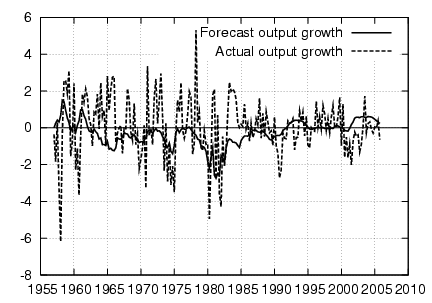
\includegraphics[scale=0.2]{plots/nok_gh_fe_y.png} & 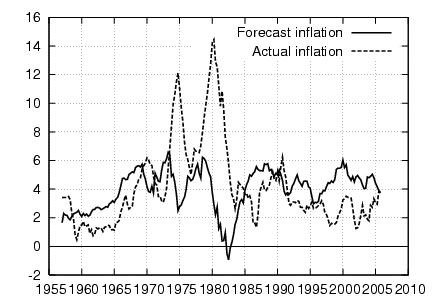
\includegraphics[scale=0.2]{plots/nok_gh_fe_pi.png} & 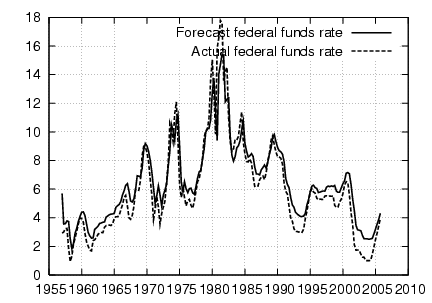
\includegraphics[scale=0.2]{plots/nok_gh_fe_r.png} \\
\multicolumn{3}{c}{Rational Expectations} \\
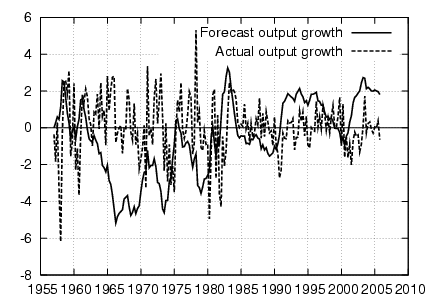
\includegraphics[scale=0.2]{plots/nok_h_fe_y.png} & 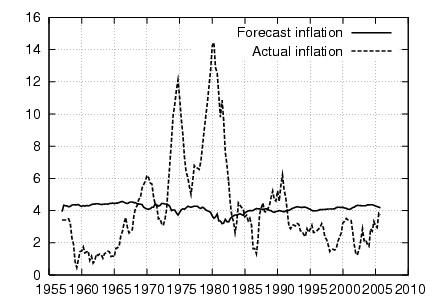
\includegraphics[scale=0.2]{plots/nok_h_fe_pi.png} & 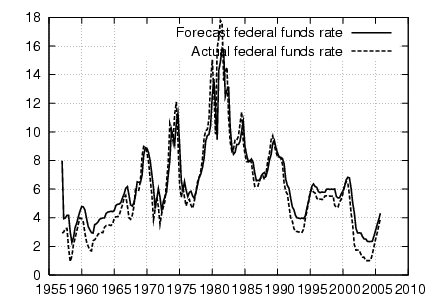
\includegraphics[scale=0.2]{plots/nok_h_fe_r.png} \\
\end{tabular}
\end{center}
\end{figure}
}

\frame
{
  \ft{Comparison}
  \bi
  \item Learning forecast errors for output and inflation are less correlated.
  \item Learning generates more volatility for inflation.
  \item Both estimates still miss inflation episodes in the 1970s.
  \ei
}

\frame
{
\begin{table}[ht]
\caption{MLE Results with Learning and Endogenous Capital}\label{tb:mle_kln}
\begin{footnotesize}
\begin{center}
\begin{tabular}{|l|c|c|c|c|} \hline
Parameter &  & Estimate & Std. Dev. & P-value \\ \hline
Learning gain & $g$ & 0.025106 & 0.002111 & 0.000000 \\ 
Habit formation & $\eta$ & 0.716807 & 0.000066 & 0.000000 \\ 
Inverse elasticity sub. & $\sigma$ & 6.424134 & 0.002669 & 0.000000 \\ 
Inverse elasticity labor supply & $\mu$ & 0.911733 & 0.002737 & 0.000000 \\ 
Cost of adjusting capital & $\phi$ & 8.821684 & 0.000867 & 0.000000 \\ 
Elasticity sub. in production & $\theta$ & 3.650960 & 0.000395 & 0.000000 \\ 
Price flexibility & $\kappa$ & 0.001962 & 0.000021 & 0.000000 \\ 
MP interest rate smoothing & $\rho_r$ & 0.877350 & 0.000137 & 0.000000 \\ 
MP feedback on output & $\psi_y$ & 0.190299 & 0.000015 & 0.000000 \\ 
MP feedback on inflation & $\psi_{\pi}$ & 0.514582 & 0.000134 & 0.000000 \\ 
Steady state inflation & $\pi^{*}$ & 0.929303 & 0.002806 & 0.000000 \\ 
Std. dev. technology shock & $\sigma_z$ & 0.947077 & 0.000021 & 0.000000 \\ 
Std. dev. investment shock & $\sigma_{\mu}$ & 0.322885 & 0.000024 & 0.000000 \\ 
Std. dev. preference shock & $\sigma_{\xi}$ & 1.402110 & 0.002658 & 0.000000 \\ 
Std. dev. interest rate shock & $\sigma_{r}$ & 0.011280 & 0.000075 & 0.000000 \\ \hline 
\multicolumn{2}{|l|}{MSE Output growth} & \multicolumn{3}{|l|}{5.324316} \\ 
\multicolumn{2}{|l|}{MSE Investment growth} & \multicolumn{3}{|l|}{147.418957} \\ 
\multicolumn{2}{|l|}{MSE Inflation} & \multicolumn{3}{|l|}{5.038744} \\ 
\multicolumn{2}{|l|}{MSE Interest rate} & \multicolumn{3}{|l|}{1.929975} \\ \hline 
\end{tabular}
\end{center}
\end{footnotesize}
\end{table}
}

\frame
{
  \ft{Results with Learning and Endogenous Capital}
  \bi
  \item Even higher statistically significant estimate for the learning gain.
  \item Habit formation is still a significant source of persistence.
  \item Taylor rule parameters look very different.
  \ei
}

\frame
{
\begin{figure}[ht]
\caption{Forecast Errors with Learning and Endogenous Capital}
\begin{center}
\begin{tabular}{cc}
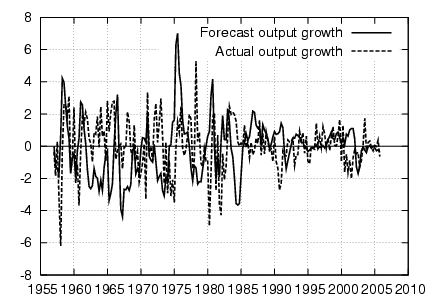
\includegraphics[scale=0.3]{plots/k_gh_fe_y.png}  & 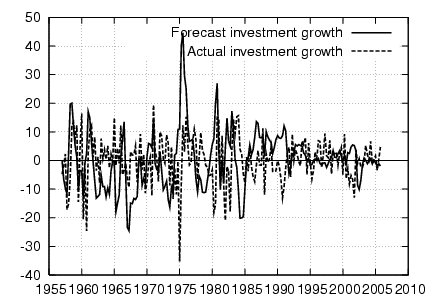
\includegraphics[scale=0.3]{plots/k_gh_fe_I.png}  \\
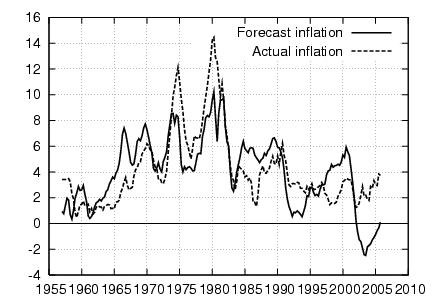
\includegraphics[scale=0.3]{plots/k_gh_fe_pi.png} & 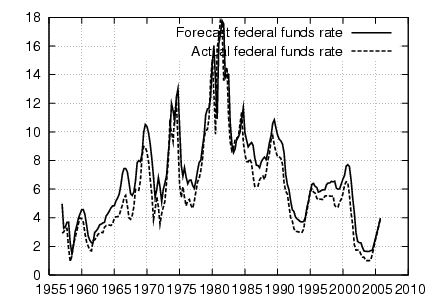
\includegraphics[scale=0.3]{plots/k_gh_fe_r.png}  \\
\end{tabular}
\end{center}
\end{figure}
}

\frame
{
\begin{figure}[ht]
\caption{Forecast Errors with No Learning and Endogenous Capital}
\begin{center}
\begin{tabular}{cc}
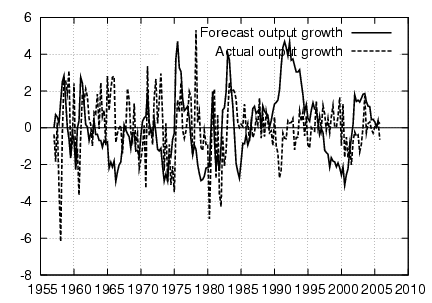
\includegraphics[scale=0.3]{plots/k_h_fe_y.png}  & 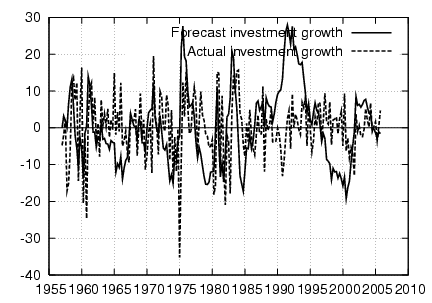
\includegraphics[scale=0.3]{plots/k_h_fe_I.png}  \\
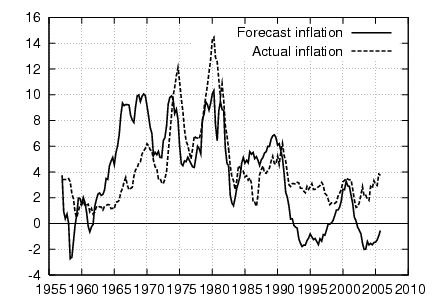
\includegraphics[scale=0.3]{plots/k_h_fe_pi.png} & 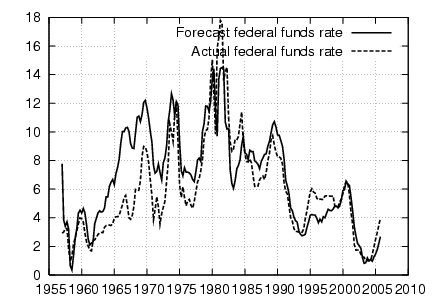
\includegraphics[scale=0.3]{plots/k_h_fe_r.png}  \\
\end{tabular}
\end{center}
\end{figure}
}

\frame
{
  \ft{Comparison}
  \bi
  \item Without learning: predicts persistent volatility throughout sample in output, investment, and inflation.
  \item With Learning: 
    \bi
    \item Correctly predicts volatility in output, investment and inflation in 1970s.
    \item Correctly predicts low volatility in output and investment from mid-1980s onward.
    \item Correctly predicts low volatility in inflation during late 1950s, early 1960s and during 1980s and 1990s.
    \ei
  \ei
}

\frame
{
  \ft{Conclusion}
  \bi
  \item Capital in the New Keynesian model has non-trivial implications for output and inflation dynamics, especially with learning.
  \item Including capital still leads to statistically significant learning gain.
  \item Capital + learning is best able to predict the changing volatility of output, investment, and inflation in the post-war period.
  \ei
}

\frame
{
  \ft{Work yet to do}
  \bi
  \item Generate impulse response functions for expectations or expectation errors.
  \item Produce plots of agents' forecast errors through the sample.  
  \item Results are currently sensitive to initial guess for MLE solution.
    \bi
    \item Maximize likelihood using simulated annealing: its been running for days.
    \ei
  \item Estimate subsamples, look for structural changes especially in monetary policy.
  \ei
}

\end{document}

